
%{{第十三回}}{第十三回}}

\chapter{秦可卿死封龙禁尉\\王熙凤协理宁国府}\label{part0017_split_000.htmlux5cux23calibre_pb_0}

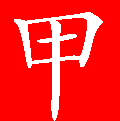
\includegraphics[width=3mm]{../Images/00002}{贾珍尚奢,岂有不请父命之理?因敬{[}老修炼{]}要紧,不问家事,故得恣意放为。}

{若明指一州名,似落《西游》□□□□□□□地,不待言可知,是光天□□□□□□□□矣。不云国名更妙,□□□□□□□□□□义之乡也。直与\ldots{}\ldots{}}

{今秦可卿托□□□□□□□□□□□□□理宁府亦□□□□□□□□□□□□□凤□□□□□□□□□□□□□□□□在封龙禁尉,写乃褒中之贬,隐去天香楼一节,是不忍下笔也。}\href{../Text/part0017_split_000.html\#lnkback_1_a}{\textsuperscript{①}}

{{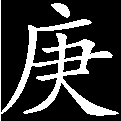
\includegraphics[width=3mm]{../Images/00004}此回可卿{[}托{]}梦阿凤,盖作者大有深意存焉。可惜生不逢时,奈何奈何!然必写出自可卿之意也,则又有他意寓焉。}}

{{荣、宁世家,未有不尊家训者。虽贾珍尚奢,岂明逆父哉?故写敬老不管,然后恣意,方见笔笔周到。}}\href{../Text/part0017_split_000.html\#lnkback_2_a}{\textsuperscript{②}}

{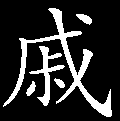
\includegraphics[width=3mm]{../Images/00005}生死穷通何处真?英明难遏是精神。微密久藏偏自露,幻中梦里语惊人。}

诗云:

一步行来错,回头已百年。古今风月鉴,多少泣黄泉!\href{../Text/part0017_split_000.html\#lnkback_3_a}{\textsuperscript{③}}

话说凤姐自贾琏送黛玉往扬州去后,心中实在无趣,每到晚间,不过和平儿说笑一回,就胡乱{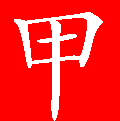
\includegraphics[width=3mm]{../Images/00002}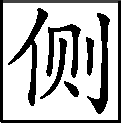
\includegraphics[width=3mm]{../Images/00011}\footnotesize \kaishu ``胡乱''二字奇。}睡了。

这日夜间,正和平儿灯下拥炉倦绣,早命浓薰绣被,二人睡下,屈指算行程该到何处,{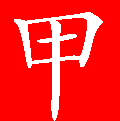
\includegraphics[width=3mm]{../Images/00002}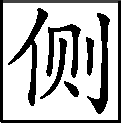
\includegraphics[width=3mm]{../Images/00011}\footnotesize \kaishu 所谓``计程今日到梁州''是也。}不知不觉已交三鼓。平儿已睡熟了。凤姐方觉星眼微朦,恍惚只见秦氏从外走了进来,含笑说道:``婶婶好睡!我今儿回去,你也不送我一程。因娘儿们素日相好,我舍不得婶婶,故来别你一别。还有一件心愿未了,非告诉婶子,别人未必中用。''{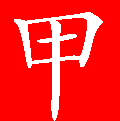
\includegraphics[width=3mm]{../Images/00002}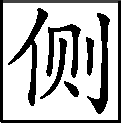
\includegraphics[width=3mm]{../Images/00011}\footnotesize \kaishu 一语贬尽贾家一族空顶冠束带者。}

凤姐听了,恍惚问道:``有何心愿?你只管托我就是了。''秦氏道:``婶婶,你是个脂粉队内的英雄,{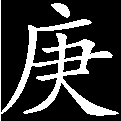
\includegraphics[width=3mm]{../Images/00004}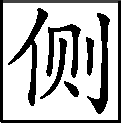
\includegraphics[width=3mm]{../Images/00011}\footnotesize \kaishu 称得起。}连那些束带顶冠的男子也不能过你,你如何连两句俗语也不晓得?常言`月满则亏,水满则溢';又道是`登高必跌重'。如今我们家赫赫扬扬,已将百载,一日倘或{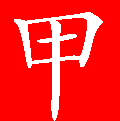
\includegraphics[width=3mm]{../Images/00002}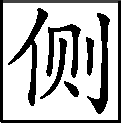
\includegraphics[width=3mm]{../Images/00011}\footnotesize \kaishu ``倘或''二字酷肖妇女口气。}乐极悲生,若应了那句`树倒猢狲散'的俗语,{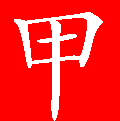
\includegraphics[width=3mm]{../Images/00002}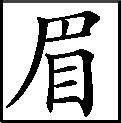
\includegraphics[width=3mm]{../Images/00010}\footnotesize \kaishu ``树倒猢狲散''之语,今犹在耳,屈指三十五年矣。哀哉伤哉,宁不恸杀!}岂不虚称了一世的诗书旧族了!''凤姐听了此话,心胸大快,十分敬畏,忙问道:``这话虑的极是,但有何法可以永保无虞?''{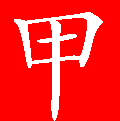
\includegraphics[width=3mm]{../Images/00002}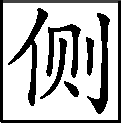
\includegraphics[width=3mm]{../Images/00011}\footnotesize \kaishu 非阿凤不明,盖今古名利场中患失之同意也。}秦氏冷笑道:``婶婶好痴也!否极泰来,荣辱自古周而复始,岂是人力能可保常的。但如今能于荣时筹画下将来衰时的世业,亦可谓常保永全了。即如今日诸事都妥,只有两件事未妥,若把此事如此一行,则日后可保永全了。''

凤姐便问何事。秦氏道:``目今祖茔虽四时祭祀,只是无一定的钱粮;第二,家塾虽立,无一定的供给。依我想来,如今盛时固不缺祭祀、供给,但将来败落之时,此二项有何出处?莫若依我定见,趁今日富贵,将祖茔附近多置田庄、房舍、地亩,以备祭祀供给之费皆出自此处,将家塾亦设于此。合同族中长幼,大家定了则例,日后按房掌管这一年的地亩、钱粮、祭祀、供给之事。如此周流,又无争竞,亦不有典卖诸弊。便是有了罪,凡物可入官,这祭祀产业连官也不入的。便败落下来,子孙回家读书务农,也有个退步,{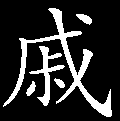
\includegraphics[width=3mm]{../Images/00005}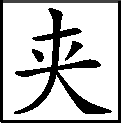
\includegraphics[width=3mm]{../Images/00012}\footnotesize \kaishu 幻情文字中忽入此等警句,提醒多少热心人。}祭祀又可永继。若目今以为荣华不绝,不思日后,终非长策。眼见不日又有一件非常喜事,真是烈火烹油、鲜花着锦之盛。要知道,也不过是瞬息的繁华,一时的欢乐,{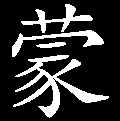
\includegraphics[width=3mm]{../Images/00006}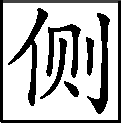
\includegraphics[width=3mm]{../Images/00011}\footnotesize \kaishu ``瞬息繁华,一时欢乐''二语,可共天下有志事业功名者同来一哭。但天生人非无所为,遇机会,成事业,留名于后世者,亦必有奇传奇遇,方能成不世之功。此亦皆苍天暗中扶助,虽有波澜,而无甚害,反觉其铮铮有声。其不成也,亦由天命。其奸人倾险之计,亦非天命不能行。其繁华欢乐,亦自天命。人于其间,知天命而存好生之心,尽己力以周旋其间,不计其功之成与否,所谓心安而理尽,又何患乎?一时瞬息,随缘遇缘,乌乎不可!}万不可忘了那`盛筵必散'\href{../Text/part0017_split_000.html\#lnkback_4_a}{\textsuperscript{④}}的俗语。此时若不早为后虑,临期只恐后悔无益了。''{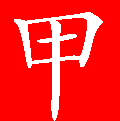
\includegraphics[width=3mm]{../Images/00002}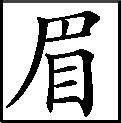
\includegraphics[width=3mm]{../Images/00010}\footnotesize \kaishu 语语见道,字字伤心,读此一段,几不知此身为何物矣。松斋。}凤姐忙问:``有何喜事?''秦氏道:``天机不可泄漏。{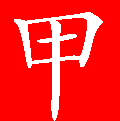
\includegraphics[width=3mm]{../Images/00002}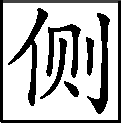
\includegraphics[width=3mm]{../Images/00011}\footnotesize \kaishu 伏的妙!}只是我与婶子好了一场,临别赠你两句话,须要记着。''因念道:

三春去后诸芳尽,各自须寻各自门。{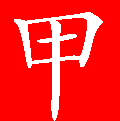
\includegraphics[width=3mm]{../Images/00002}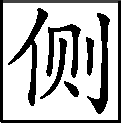
\includegraphics[width=3mm]{../Images/00011}\footnotesize \kaishu 此句令批书人哭死。 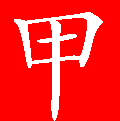
\includegraphics[width=3mm]{../Images/00002}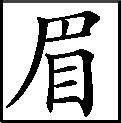
\includegraphics[width=3mm]{../Images/00010}\footnotesize \kaishu 不必看完,见此二句,即欲堕泪。梅溪。}

凤姐还欲问时,只听二门上传事云板连叩四下,{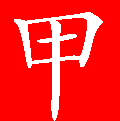
\includegraphics[width=3mm]{../Images/00002}正是丧音。}\href{../Text/part0017_split_000.html\#lnkback_5_a}{\textsuperscript{⑤}}将凤姐惊醒。人回:``东府蓉大奶奶没了。''凤姐闻听,吓了一身冷汗,出了一回神,只得忙忙的穿衣服,往王夫人处来。

彼时合家皆知,无不纳罕,都有些疑心。{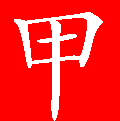
\includegraphics[width=3mm]{../Images/00002}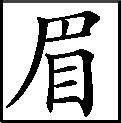
\includegraphics[width=3mm]{../Images/00010}\footnotesize \kaishu 九个字写尽天香楼事,是不写之写。 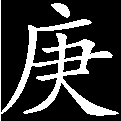
\includegraphics[width=3mm]{../Images/00004}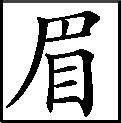
\includegraphics[width=3mm]{../Images/00010}\footnotesize \kaishu 可从此批。}那长一辈的想他素日孝顺,平一辈的想他平日和睦亲密,{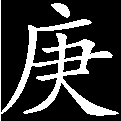
\includegraphics[width=3mm]{../Images/00004}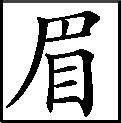
\includegraphics[width=3mm]{../Images/00010}\footnotesize \kaishu 松斋云:好笔力。此方是文字佳处。}下一辈的想他素日慈爱,以及家中仆从老小想他素日怜贫惜贱、慈老爱幼{{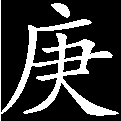
\includegraphics[width=3mm]{../Images/00004}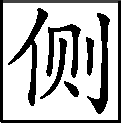
\includegraphics[width=3mm]{../Images/00011}\footnotesize \kaishu 八字乃为上人{(之)}{[}者{]}当铭于五衷。}}之恩,莫不悲嚎痛哭者。{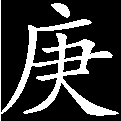
\includegraphics[width=3mm]{../Images/00004}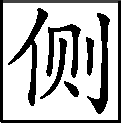
\includegraphics[width=3mm]{../Images/00011}\footnotesize \kaishu 老健。}

闲言少叙,却说宝玉因近日林黛玉回去,剩得自己孤凄,也不和人顽耍,{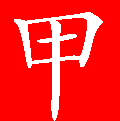
\includegraphics[width=3mm]{../Images/00002}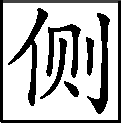
\includegraphics[width=3mm]{../Images/00011}\footnotesize \kaishu 与凤姐反对。◇淡淡写来,方是二人自幼气味相投,可知后文皆非突然文字。}每到晚间,便索然睡了。如今从梦中听见说秦氏死了,连忙翻身爬起来,只觉心中似戮了一刀的不忍,``哇''的一声,喷出一口血来。{{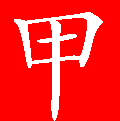
\includegraphics[width=3mm]{../Images/00002}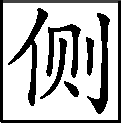
\includegraphics[width=3mm]{../Images/00011}\footnotesize \kaishu 宝玉早已看定,可继家务事者可卿也,今闻死了,大失所望。急火攻心,焉得不有此血?为玉一叹! 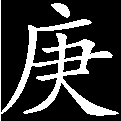
\includegraphics[width=3mm]{../Images/00004}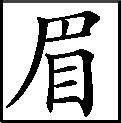
\includegraphics[width=3mm]{../Images/00010}\footnotesize \kaishu 如{(在)}{[}此{]}总是淡描轻写,全无痕迹,方见得有生以来,天分中自然所赋之性如此,非因色所{(感)}{[}惑{]}也。}}袭人等慌慌忙忙上来搊扶,问是怎么样,又要回贾母来请大夫。宝玉笑道:``不用忙,不相干,{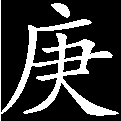
\includegraphics[width=3mm]{../Images/00004}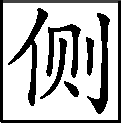
\includegraphics[width=3mm]{../Images/00011}\footnotesize \kaishu 又淡淡抹去。}这是急火攻心,{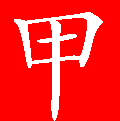
\includegraphics[width=3mm]{../Images/00002}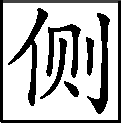
\includegraphics[width=3mm]{../Images/00011}\footnotesize \kaishu 如何自己说出来了?}血不归经。''说着便爬起来,要衣服换了,来见贾母,即时要过去。袭人见他如此,心中虽放不下,又不敢拦,只是由他罢了。贾母见他要去,因说:``才咽气的人,那里不干净;二则夜里风大,等明早再去不迟。''宝玉那里肯依。贾母命人备车,多派跟从人役,拥护前来。

一直到了宁国府前,只见府门洞开,两边灯笼照如白昼,乱烘烘人来人往,里面哭声摇山振岳。{\includegraphics[width=3mm]{../Images/00002}\includegraphics[width=3mm]{../Images/00011}\footnotesize \kaishu 写大族之丧,如此起绪。}宝玉下了车,忙忙奔至停灵之室,痛哭一番。然后见过尤氏。谁知尤氏正犯了胃疼旧疾,睡在床上。{{\includegraphics[width=3mm]{../Images/00002}\includegraphics[width=3mm]{../Images/00011}\footnotesize \kaishu 妙!非此何以出阿凤! \includegraphics[width=3mm]{../Images/00004}\includegraphics[width=3mm]{../Images/00011}\footnotesize \kaishu 紧处愈紧,密处愈密。 \includegraphics[width=3mm]{../Images/00004}\includegraphics[width=3mm]{../Images/00010}\footnotesize \kaishu 所谓层峦叠翠之法也。野史中从无此法。即观者到此,亦{(为)}{[}谓{]}写秦氏未必全到,岂料更又写一尤氏哉!}}然后又出来见贾珍。彼时贾代儒带领贾敕、贾效、贾敦、贾赦、贾政、贾琮、贾?、贾珩、贾珖、贾琛、贾琼、贾璘、贾蔷、贾菖、贾菱、贾芸、贾芹、贾蓁、贾萍、贾藻、贾蘅、贾芬、贾芳、贾兰、贾菌、贾芝等{\includegraphics[width=3mm]{../Images/00004}\includegraphics[width=3mm]{../Images/00011}\footnotesize \kaishu 将贾族约略一总,观者方不惑。}都来了。贾珍哭的泪人一般,{\includegraphics[width=3mm]{../Images/00002}\includegraphics[width=3mm]{../Images/00011}\footnotesize \kaishu 可笑。如丧考妣,此作者刺心笔也。}正和贾代儒等说道:``合家大小,远亲近友,谁不知我这媳妇比儿子还强十倍。如今伸腿去了,可见这长房内绝灭无人了。''说着又哭起来。众人忙劝道:``人已辞世,哭也无益,且商议如何料理要紧。''{\includegraphics[width=3mm]{../Images/00004}\includegraphics[width=3mm]{../Images/00011}\footnotesize \kaishu 淡淡一句,勾出贾珍多少文字来。}贾珍拍手道:``如何料理,不过尽我所有罢了!''{\includegraphics[width=3mm]{../Images/00005}\includegraphics[width=3mm]{../Images/00012}\footnotesize \kaishu ``尽我所有'',为媳妇是非礼之谈,父母又将何以待之?故前此有恶奴酒后狂言,及今复见此语,含而不露,吾不能为贾珍隐讳。}

正说着,只见秦业、秦钟并尤氏的几个眷属{\includegraphics[width=3mm]{../Images/00002}\includegraphics[width=3mm]{../Images/00011}\footnotesize \kaishu 伏后文。}尤氏姊妹也都来了。贾珍便命贾琼、贾琛、贾璘、贾蔷四个人去陪客,一面吩咐去请钦天监阴阳司来择日,推准停灵七七四十九日,三日后开丧送讣闻。这四十九日,单请一百单八众禅僧在大厅上拜大悲忏,超度前亡后化诸魂,以免亡者之罪;另设一坛于天香楼上,{\includegraphics[width=3mm]{../Images/00002}\includegraphics[width=3mm]{../Images/00011}\footnotesize \kaishu 删。却是未删之笔。}是九十九位全真道士,打四十九日解冤洗业醮。然后停灵于会芳园中,灵前另有五十众高僧、五十众高道,对坛按七作好事。那贾敬闻得长孙媳妇死了,因自为早晚就要飞升,{{\includegraphics[width=3mm]{../Images/00004}\includegraphics[width=3mm]{../Images/00011}\footnotesize \kaishu 可笑可叹。古今之儒,中途多惑老佛。王隐梅云:``若能再加东坡十年寿,亦能跳出这圈子来。''斯言信矣。 }\includegraphics[width=3mm]{../Images/00006}\includegraphics[width=3mm]{../Images/00011}\footnotesize \kaishu ``就要飞升''的``要'',用得的当。凡``要''者,则身心急切;急切之者,百事无成。正为后文作引线。}如何肯又回家染了红尘,将前功尽弃呢,因此并不在意,只凭贾珍料理。

贾珍见父亲不管,亦发恣意奢华。看板时,几副杉木板皆不中用。可巧薛蟠来吊问,因见贾珍寻好板,便说道:``我们木店里有一副,叫做什么樯木,{\includegraphics[width=3mm]{../Images/00002}\includegraphics[width=3mm]{../Images/00010}\footnotesize \kaishu 樯者,舟具也。所谓``人生若泛舟''而已,宁不可叹!}出在潢海铁网山上,{\includegraphics[width=3mm]{../Images/00002}\includegraphics[width=3mm]{../Images/00011}\footnotesize \kaishu 所谓迷津易堕,尘网难逃也。}作了棺材,万年不坏。这还是当年先父带来,原系义忠亲王老千岁要的,因他坏了事,{\includegraphics[width=3mm]{../Images/00006}\includegraphics[width=3mm]{../Images/00011}\footnotesize \kaishu ``坏了事''等字毒极,写尽势利场中故套。}就不曾拿去。现今还封在店里,也没人出价敢买。你若要,就抬来罢了。''贾珍听了,喜之不禁,即命人抬来。大家看时,只见帮底皆厚八寸,纹若槟榔,味若檀麝,以手扣之,玎珰如金玉。大家都奇异称赏。贾珍笑道:``价值几何?''薛蟠笑道:``拿一千两银子来,只怕也没处买去。什么价不价,赏他们几两工银就是了。''{\includegraphics[width=3mm]{../Images/00002}\includegraphics[width=3mm]{../Images/00011}\footnotesize \kaishu 的是阿呆兄口气。}贾珍听说,忙谢不尽,即命解锯糊漆。贾政因劝道:``此物恐非常人可享者,{\includegraphics[width=3mm]{../Images/00002}\includegraphics[width=3mm]{../Images/00011}\footnotesize \kaishu 政老有深意存焉。}殓以上等杉木也就是了。''{{{\includegraphics[width=3mm]{../Images/00002}\includegraphics[width=3mm]{../Images/00011}\footnotesize \kaishu 夹写贾政。 \includegraphics[width=3mm]{../Images/00002}\includegraphics[width=3mm]{../Images/00010}\footnotesize \kaishu 写个个皆知,全无安逸之笔,深得《金瓶》}壸{奥!}}}此时贾珍恨不能代秦氏之死,这话如何肯听。{\includegraphics[width=3mm]{../Images/00006}\includegraphics[width=3mm]{../Images/00011}\footnotesize \kaishu ``代秦氏死''等句,总是填实前文。}

因忽又听得秦氏之丫鬟名唤瑞珠者,见秦氏死了,他也触柱而亡。{\includegraphics[width=3mm]{../Images/00002}\includegraphics[width=3mm]{../Images/00011}\footnotesize \kaishu 补天香楼未删之文。}此事可罕,合族中人也都称赞。贾珍遂以孙女之礼殡殓,一并停灵于会芳园之登仙阁。小丫鬟名宝珠者,因见秦氏身无所出,乃甘心愿为义女,誓任摔丧驾灵之任。贾珍喜之不禁,即时传下:从此皆呼宝珠为小姐。那宝珠按未嫁女之丧,在灵前哀哀欲绝。{\includegraphics[width=3mm]{../Images/00002}\includegraphics[width=3mm]{../Images/00011}\footnotesize \kaishu 非恩惠爱人,那能如是?惜哉可卿,惜哉可卿!}于是,合族人丁并家下诸人,都各遵旧制行事,自不敢紊乱。{\includegraphics[width=3mm]{../Images/00002}\includegraphics[width=3mm]{../Images/00011}\footnotesize \kaishu 两句写尽大家。 }\includegraphics[width=3mm]{../Images/00009}\includegraphics[width=3mm]{../Images/00012}{\footnotesize \kaishu 转叠法,叙前文未及。}

贾珍因想着贾蓉不过是个黉门监,{\includegraphics[width=3mm]{../Images/00004}\includegraphics[width=3mm]{../Images/00011}\footnotesize \kaishu 又起波澜,却不突然。}灵幡经榜上写时不好看,便是执事也不多,因此心下甚不自在。{\includegraphics[width=3mm]{../Images/00002}\includegraphics[width=3mm]{../Images/00011}\footnotesize \kaishu 善起波澜。}可巧这日正是首七第四日,早有大明宫掌宫内相戴权,{\includegraphics[width=3mm]{../Images/00002}\includegraphics[width=3mm]{../Images/00011}\footnotesize \kaishu 妙!大权也。}先备了祭礼遣人抬来,次后坐了大轿,打伞鸣锣,亲来上祭。贾珍忙接着,让至逗蜂轩{\includegraphics[width=3mm]{../Images/00002}\includegraphics[width=3mm]{../Images/00011}\footnotesize \kaishu 轩名可思。}献茶。贾珍心中打算定了主意,因而趁便就说要与贾蓉蠲个前程的话。戴权会意,因笑道:``想是为丧礼上风光些?''{\includegraphics[width=3mm]{../Images/00002}\includegraphics[width=3mm]{../Images/00011}\footnotesize \kaishu 得内相机括之快如此。}贾珍忙笑道:``老内相所见不差。''戴权道:``事倒凑巧,正有个美缺。如今三百员龙禁尉短了两员,昨儿襄阳侯的兄弟老三来求我,现拿了一千五百两银子,送到我家里。你知道,咱们都是老相与,不拘怎么样,看着他爷爷的分上,胡乱应了。{\includegraphics[width=3mm]{../Images/00002}\includegraphics[width=3mm]{../Images/00011}\footnotesize \kaishu 忙中写闲。}还剩了一个缺,谁知永兴节度使冯胖子来求,要与他孩子蠲,我就没工夫应他。既是咱们的孩子{\includegraphics[width=3mm]{../Images/00002}\includegraphics[width=3mm]{../Images/00011}\footnotesize \kaishu 奇谈,画尽阉官口吻。}要蠲,快写个履历来。''贾珍听说,忙吩咐:``快命书房里人恭敬写了大爷的履历来。''小厮不敢怠慢,去了一刻,便拿了一张红纸来与贾珍。贾珍看了,忙送与戴权。戴权看时,上面写道:

江南江宁府江宁县监生贾蓉,年二十岁。曾祖,原任京营节度使世袭一等神威将军贾代化;祖,乙卯科进士贾敬;父,世袭三品爵威烈将军贾珍。

戴权看了,回手便递与一个贴身的小厮收了,说道:``回来送与户部堂官老赵,说我拜上他,起一张五品龙禁尉的票,再给个执照,就把那履历填上,明儿我来兑银子送去。''小厮答应了,戴权也就告辞了。贾珍十分款留不住,只得送出府门。临上轿,贾珍因问:``银子还是我到部兑,还是一并送入老内相府中?''戴权道:``若到部里,你又吃亏了。不如平准一千二百银子,送到我家里就完了。''贾珍感谢不尽,只说:``待服满后,亲带小犬到府叩谢。''于是作别。

接着,又听喝道之声,原来是忠靖侯史鼎的夫人来了。{{\includegraphics[width=3mm]{../Images/00002}\includegraphics[width=3mm]{../Images/00011}\footnotesize \kaishu 史小姐湘云消息也。} \includegraphics[width=3mm]{../Images/00005}\includegraphics[width=3mm]{../Images/00012}\footnotesize \kaishu 伏史湘云一笔。}\href{../Text/part0017_split_000.html\#lnkback_6_a}{\textsuperscript{⑥}}{ \includegraphics[width=3mm]{../Images/00009}\includegraphics[width=3mm]{../Images/00012}\footnotesize \kaishu 伏下文史湘云。}王夫人、邢夫人、凤姐等刚迎至上房,又见锦乡侯、川宁侯、寿山伯三家祭礼摆在灵前。少时,三家下轿,贾政等忙接上大厅。如此亲朋你来我去,也不能胜数。只这四十九日,{\includegraphics[width=3mm]{../Images/00004}\includegraphics[width=3mm]{../Images/00011}\footnotesize \kaishu 就简去繁。}宁国府街上一条白漫漫人来人往,{\includegraphics[width=3mm]{../Images/00002}\includegraphics[width=3mm]{../Images/00011}\footnotesize \kaishu 是有服亲友并家下人丁之盛。}花簇簇宦去官来。{\includegraphics[width=3mm]{../Images/00002}\includegraphics[width=3mm]{../Images/00011}\footnotesize \kaishu 是来往祭吊之盛。}

贾珍命贾蓉次日换了吉服,领凭回来。灵前供用执事等物,俱按五品职例。灵牌疏上皆写``天朝诰授贾门秦氏恭人之灵位''。会芳园的临街大门洞开,现在两边起了鼓乐厅,两班青衣按时奏乐,一对对执事摆的刀斩斧齐。更有四面朱红销金大字牌对竖在门外,上面大书:

防护内廷紫禁道 御前侍卫龙禁尉。

对面高起着宣坛,僧道对坛榜文,榜上大书:

世袭宁国公冢孙妇、防护内廷御前侍卫龙禁尉贾门秦氏恭人之丧。{\includegraphics[width=3mm]{../Images/00004}\includegraphics[width=3mm]{../Images/00010}\footnotesize \kaishu 贾珍是乱费,可卿却实如此。}四大部州至中之地,奉天承运太平之国,{\includegraphics[width=3mm]{../Images/00004}\includegraphics[width=3mm]{../Images/00010}\footnotesize \kaishu 奇文。若明指一州名,似落《西游》之套,故曰至中之地,不待言可知是光天化日、仁风德雨之下矣。不云国名更妙,可知是尧街舜巷、衣冠礼义之乡矣。直与第一回呼应相接。}总理虚无寂静教门僧录司正堂万虚、总理元始三一教门道录司正堂叶生等,敬谨修斋,朝天叩佛。

以及------

恭请诸伽蓝、揭谛、功曹等神,圣恩普锡,神威远镇,四十九日消灾洗业平安水陆道场。

诸如等语,馀者亦不消烦记。

只是贾珍虽然此时心意满足,{\includegraphics[width=3mm]{../Images/00006}\includegraphics[width=3mm]{../Images/00011}\footnotesize \kaishu 可笑。}但里头尤氏又犯了旧疾,不能料理事务,惟恐各诰命来往,亏了礼数,怕人笑话,因此心中不自在。当下正忧虑时,因宝玉{\includegraphics[width=3mm]{../Images/00002}\includegraphics[width=3mm]{../Images/00011}\footnotesize \kaishu 余正思如何高搁起玉兄了。}在侧问道:``事事都算安贴了,大哥哥还愁什么?''贾珍见问,忙将里面无人的话说了出来。宝玉听说笑道:``这有何难,我荐一个人{\includegraphics[width=3mm]{../Images/00002}\includegraphics[width=3mm]{../Images/00011}\footnotesize \kaishu 荐凤姐须得宝玉,俱龙华会上人也。}与你权理这一个月的事,管必妥当。''贾珍忙问:``是谁?''宝玉见座间还有许多亲友,不便明言,走至贾珍耳边说了两句。贾珍听了喜不自禁,连忙起身笑道:``果然安贴,如今就去。''说着拉了宝玉,辞了众人,便往上房里来。

可巧这日非正经日期,亲友来的少,里面不过几位近亲堂客,邢夫人、王夫人、凤姐并合族中的内眷陪坐。有人报说:``大爷进来了。''吓的众婆娘``唿''的一声,往后藏之不迭,{{\includegraphics[width=3mm]{../Images/00002}\includegraphics[width=3mm]{../Images/00011}\footnotesize \kaishu {(数)}{[}素{]}日行止可知。作者自是笔笔不空,批者亦字字留神之至矣。}}独凤姐款款站了起来。{\includegraphics[width=3mm]{../Images/00004}\includegraphics[width=3mm]{../Images/00011}\footnotesize \kaishu 又写凤姐。}贾珍此时也有些病症在身,二则过于悲痛了,因拄了拐踱了进来。邢夫人等因说道:``你身上不好,又连日事多,该歇歇才是,又进来做什么?''贾珍一面扶拐,{\includegraphics[width=3mm]{../Images/00004}\includegraphics[width=3mm]{../Images/00011}\footnotesize \kaishu 一丝不乱。}扎挣着要蹲身跪下请安道乏。邢夫人等忙叫宝玉搀住,命人挪椅子来与他坐。贾珍断不肯坐,因勉强陪笑道:``侄儿进来有一件事要恳求二位婶婶并大妹妹。''邢夫人等忙问:``什么事?''贾珍忙笑道:``婶婶自然知道,如今孙子媳妇没了,侄儿媳妇偏又病倒,我看里头着实不成个体统。怎么屈尊大妹妹一个月,{\includegraphics[width=3mm]{../Images/00004}\includegraphics[width=3mm]{../Images/00011}\footnotesize \kaishu 不见突然。}在这里料理料理,我就放心了。''{\includegraphics[width=3mm]{../Images/00004}\includegraphics[width=3mm]{../Images/00011}\footnotesize \kaishu 阿凤此刻心痒矣。}邢夫人笑道:``原来为这个。你大妹妹现在你二婶子家,只和你二婶子说就是了。''王夫人忙道:``他一个小孩子{\includegraphics[width=3mm]{../Images/00004}\includegraphics[width=3mm]{../Images/00011}\footnotesize \kaishu 三字愈令人可爱可怜。}家,何曾经过这样事,倘或料理不清,反叫人笑话,倒是再烦别人好。''贾珍笑道:``婶子的意思侄儿猜着了,是怕大妹妹劳苦了。若说料理不开,我包管必料理的开,便是错一点儿,别人看着还是不错的。从小儿大妹妹顽笑着就有杀伐决断,{\includegraphics[width=3mm]{../Images/00004}\includegraphics[width=3mm]{../Images/00011}\footnotesize \kaishu 阿凤身份。}如今出了阁,又在那府里办事,越发历练老成了。我想了这几日,除了大妹妹再无人了。婶婶不看侄儿、侄儿媳妇的分上,只看死了的分上罢!''说着滚下泪来。{\includegraphics[width=3mm]{../Images/00004}\includegraphics[width=3mm]{../Images/00011}\footnotesize \kaishu 有笔力。}

王夫人心中怕的是凤姐未经过丧事,怕他料理不清,惹人笑话。今见贾珍苦苦的说到这步田地,心中已活了几分,却又眼看着凤姐出神。那凤姐素日最喜揽事办,好卖弄才干,虽然当家妥当,也因未办过婚丧大事,恐人还不服,巴不得遇见这事。今日见贾珍如此一来,他心中早已欢喜。先见王夫人不允,后见贾珍说的情真,王夫人有活动之意,便向王夫人道:``大哥哥说的这么恳切,太太就依了罢。''王夫人悄悄的道:``你可能么?''凤姐道:``有什么不能的。外面的大事大哥哥{\includegraphics[width=3mm]{../Images/00004}\includegraphics[width=3mm]{../Images/00011}\footnotesize \kaishu 王夫人是悄言,凤姐是响应,故称``大哥哥''。}已经料理清了,{\includegraphics[width=3mm]{../Images/00004}\includegraphics[width=3mm]{../Images/00011}\footnotesize \kaishu 已得三昧矣。}不过是里头照管照管,便是我有不知道的,问问太太就是了。''{\includegraphics[width=3mm]{../Images/00002}\includegraphics[width=3mm]{../Images/00011}\footnotesize \kaishu 胸中成见已有之语。}王夫人见说的有理,便不则声。贾珍见凤姐允了,又陪笑道:``也管不得许多了,横竖要求大妹妹辛苦辛苦。我这里先与妹妹行礼,等事完了,我再到那府里去谢。''说着,就作揖下去,凤姐儿还礼不迭。

贾珍便忙向袖中取了宁国府对牌出来,命宝玉送与凤姐,又说:``妹妹爱怎么样就怎么样,要什么只管拿这个取去,也不必问我。只别存心替我省钱,只要好看为上;二则也要与那府里一样待人才好,不要存心怕人抱怨。只这两件外,我再没不放心的了。''凤姐不敢就接牌,{\includegraphics[width=3mm]{../Images/00005}\includegraphics[width=3mm]{../Images/00012}\footnotesize \kaishu 凡有本领者断不越礼。接牌小事而必待命于王夫人也,诚家道之规范,亦天下之规范也。看是书者不可草草从事。}只看着王夫人。王夫人道:``你哥哥既这么说,你就照看照看罢了。只是别自作主意,有了事,打发人问你哥哥、嫂子要紧。''宝玉早向贾珍手里接过对牌来,强递与凤姐了。贾珍又问:``妹妹还是住在这里,还是天天来呢?若是天天来,越发辛苦了。不如我这里赶着收拾出一个院落来,妹妹住过这几日倒安稳。''凤姐笑道:``不用。{\includegraphics[width=3mm]{../Images/00002}\includegraphics[width=3mm]{../Images/00011}\footnotesize \kaishu 二字句,有神。}那边也离不得我,倒是天天来的好。''贾珍听说,只得罢了。然后又说了一回闲话,方才出去。

一时女眷散后,王夫人因问凤姐:``你今儿怎么样?''凤姐儿道:``太太只管请回去,我须得先理出一个头绪来,才回去得呢。''王夫人听说,便先同邢夫人等回去,不在话下。

这里凤姐儿来至三间一所抱厦内坐了,因想:头一件是人口混杂,遗失东西;第二件,事无专执,临期推委;第三件,需用过费,滥支冒领;第四件,任无大小,苦乐不均;第五件,家人豪纵,有脸者不服钤束,无脸者不能上进。{\includegraphics[width=3mm]{../Images/00002}\includegraphics[width=3mm]{../Images/00010}\footnotesize \kaishu 旧族后辈受此五病者颇多,余家更甚。三十年前事见书于三十年后,令余悲恸血泪盈面。 \includegraphics[width=3mm]{../Images/00004}\includegraphics[width=3mm]{../Images/00010}\footnotesize \kaishu 读五件事未完,余不禁失声大哭,三十年前作书人在何处耶?}此五件实是宁国府中风俗。不知凤姐如何处治,且听下回分解。{\includegraphics[width=3mm]{../Images/00002}\includegraphics[width=3mm]{../Images/00010}\footnotesize \kaishu 此回只十页,因删去``天香楼''一节,少去四五页也。}正是:{\includegraphics[width=3mm]{../Images/00005}\includegraphics[width=3mm]{../Images/00012}\footnotesize \kaishu 五件事若能如法整理得当,岂独家庭,国家天下治之不难。}

金紫万千谁治国,裙钗一二可齐家。

{\includegraphics[width=3mm]{../Images/00002}``秦可卿淫丧天香楼'',作者用史笔也。老朽因有魂托凤姐贾家后事二件,嫡是安富尊荣坐享人能想得到处。其事虽未漏,其言其意则令人悲切感服,姑赦之,因命芹溪删去。}

{\includegraphics[width=3mm]{../Images/00004}通回将可卿如何死故隐去,是大发慈悲心也,叹叹!壬午春。}\href{../Text/part0017_split_000.html\#lnkback_7_a}{\textsuperscript{⑦}}

{\includegraphics[width=3mm]{../Images/00005}总评:借可卿之死,又写出情之变态,上下大小,男女老少,无非情感而生情。且又藉凤姐之梦,更化就幻空中一片贴切之情,所谓寂然不动,感而遂通。所感之象,所动之萌,深浅诚伪,随种必报,所谓幻者此也,情者亦此也。何非幻,何非情?情即是幻,幻即是情,明眼者自见。}

{\href{../Text/part0017_split_000.html\#navto_1_a}{①}按:底本此页被对角撕去,缺字较多,因与庚辰本相关批语内容类似,可参看,缺字不补。}

{\href{../Text/part0017_split_000.html\#navto_2_a}{②}以上二条庚辰本批语及题诗,原在第二册目录后加页上,参照甲戌本回前评移此。}

{\href{../Text/part0017_split_000.html\#navto_3_a}{③}底本自此回至第十六回,回前均有``诗云(曰)''字样而无诗。此诗据庚辰本补。}

{\href{../Text/part0017_split_000.html\#navto_4_a}{④}原作``盛筵不散'',除戚本``不''改为``必''外,馀本均同。一般认为,``不''是``必''之讹,本书及其他古籍均有误例。按此语疑为类似``盛筵不散,终须一散''的俗语的半句,与下文第七十二回写司棋与表弟相约``不娶不嫁''用法相近(``不娶不嫁''显为``非卿不娶非君不嫁''的省略,并非打算单身)。因别无佐证,暂依戚本改。}

{\href{../Text/part0017_split_000.html\#navto_5_a}{⑤}``正是丧音'',己、庚、戚、蒙等本无此语,当系批语混入正文。}

{\href{../Text/part0017_split_000.html\#navto_6_a}{⑥}己、庚本作``伏史湘云''并混入正文。}

{\href{../Text/part0017_split_000.html\#navto_7_a}{⑦}甲、庚本这两条批语,均批于回末空白处,但其性质并非总评,而属于侧批或眉批一类。}
